\bta{力学综合题(上)}
\begin{enumerate}
\renewcommand{\labelenumi}{\arabic{enumi}.}
% A(\Alph) a(\alph) I(\Roman) i(\roman) 1(\arabic)
%设定全局标号series=example	%引用全局变量resume=example
%[topsep=-0.3em,parsep=-0.3em,itemsep=-0.3em,partopsep=-0.3em]
%可使用leftmargin调整列表环境左边的空白长度 [leftmargin=0em]
\item
\exwhere{$ 2019 $ 年 $ 4 $ 月浙江物理选考}
某砂场为提高运输效率,研究砂粒下滑的高度与砂粒在传送带上运
动的关系,建立如图所示的物理模型。竖直平面内有一倾角$ \theta =37 ^{ \circ } $的直轨道 $ AB $,其下方右侧放置
一水平传送带,直轨道末端 $ B $ 与传送带间距可近似为零,但允许砂粒通过。转轮半径 $ R=0.4 \ m $、
转轴间距 $ L=2 \ m $ 的传送带以恒定的线速度逆时针转动,转轮最低点离地面的高度 $ H=2.2 \ m $。现将
一小物块放在距离传送带高 $ h $ 处静止释放,假设小物块从直轨道 $ B $ 端运动到达传送带上 $ C $ 点
时,速度大小不变,方向变为水平向右。已知小物块与直轨道和传送带间的动摩擦因数均为$ \mu =0.5 $。
($ \sin 37 ^{ \circ } =0.6 $)

\begin{enumerate}
\renewcommand{\labelenumi}{\arabic{enumi}.}
% A(\Alph) a(\alph) I(\Roman) i(\roman) 1(\arabic)
%设定全局标号series=example	%引用全局变量resume=example
%[topsep=-0.3em,parsep=-0.3em,itemsep=-0.3em,partopsep=-0.3em]
%可使用leftmargin调整列表环境左边的空白长度 [leftmargin=0em]
\item
若 $ h=2.4 \ m $,求小物块到达 $ B $ 端时速度的大小;
\item 
若小物块落到传送带左侧地面,求 $ h $ 需要满足的条件;
\item 
改变小物块释放的高度 $ h $,小物块从传送带的 $ D $ 点水平向右抛出,求小物块落地点到 $ D $ 点的
水平距离 $ x $ 与 $ h $ 的关系式及 $ h $ 需要满足的条件。




\end{enumerate}
\begin{figure}[h!]
\flushright
\includesvg[width=0.55\linewidth]{picture/svg/GZ-3-tiyou-0375}
\end{figure}


\banswer{
\begin{enumerate}
\renewcommand{\labelenumi}{\arabic{enumi}.}
% A(\Alph) a(\alph) I(\Roman) i(\roman) 1(\arabic)
%设定全局标号series=example	%引用全局变量resume=example
%[topsep=-0.3em,parsep=-0.3em,itemsep=-0.3em,partopsep=-0.3em]
%可使用leftmargin调整列表环境左边的空白长度 [leftmargin=0em]
\item
$ 4\ m/s $
\item 
$ h < 3.0 \ m $
\item 
$ h \neq 3.6 \ m $
\end{enumerate}


}



\newpage
\item 
\exwhere{$ 2019 $ 年北京卷}
雨滴落到地面的速度通常仅为几米每秒,这与雨滴下落过程中受到空气阻
力有关。雨滴间无相互作用且雨滴质量不变,重力加速度为 $ g $。
\begin{enumerate}
\renewcommand{\labelenumi}{\arabic{enumi}.}
% A(\Alph) a(\alph) I(\Roman) i(\roman) 1(\arabic)
%设定全局标号series=example	%引用全局变量resume=example
%[topsep=-0.3em,parsep=-0.3em,itemsep=-0.3em,partopsep=-0.3em]
%可使用leftmargin调整列表环境左边的空白长度 [leftmargin=0em]
\item
质量为 $ m $ 的雨滴由静止开始,下落高度 $ h $ 时速度为 $ u $,求这一过程中克服空气阻力所做的功
$ W_{f} = $ \tk{$W_{f}=m g h-\frac{1}{2} m u^{2}$} 。




\item 
将雨滴看作半径为 $ r $ 的球体,设其竖直落向地面的过程中所受空气阻力 $ f=k r^{2} v^{2} $,其中 $ v $ 是雨
滴的速度,$ k $ 是比例系数。
\begin{figure}[h!]
\centering
\includesvg[width=0.23\linewidth]{picture/svg/GZ-3-tiyou-0376}
\end{figure}

\begin{enumerate}
\renewcommand{\labelenumiii}{\alph{enumiii}.}
% A(\Alph) a(\alph) I(\Roman) i(\roman) 1(\arabic)
%设定全局标号series=example	%引用全局变量resume=example
%[topsep=-0.3em,parsep=-0.3em,itemsep=-0.3em,partopsep=-0.3em]
%可使用leftmargin调整列表环境左边的空白长度 [leftmargin=0em]
\item
设雨滴的密度为$ \rho $,推导雨滴下落趋近的最大速度 $ v_{m} $ 与半径 $ r $ 的关系式 \tk{$v_{m}=\sqrt{\frac{\pi r \rho g}{3 k}}$} ;

\item 
示意图中画出了半径为 $ r_{1} $、$ r_{2} $($ r_{1} > r_{2} $)的雨滴在空气中无初速下落的 $ v - t $ 图线,其中 \tk{①} 
对应半径为 $ r_{1} $ 的雨滴(选填①、②);若不计空气阻力,请在图中画出雨滴无初速下落的 $ v $–$ t $ 图
线。

%答案图像
%\includesvg[width=0.23\linewidth]{picture/svg/GZ-3-tiyou-0377} 



\end{enumerate}



\item 
由于大量气体分子在各方向运动的几率相等,其对静止雨滴的作用力为零。将雨滴简化为垂
直于运动方向面积为 $ S $ 的圆盘,证明:圆盘以速度 $ v $ 下落时受到的空气阻力 $ f \propto v^{2} $(提示:设单位
体积内空气分子数为 $ n $,空气分子质量为 $ m_{0} $)。

\banswer{
解得 $: \quad f=2 S v^{2} n m_{0} \propto v^{2}$
}




\end{enumerate}




\newpage
\item 
\exwhere{$ 2019 $ 年物理天津卷}
完全由我国自行设计、建造的国产新型航空母舰已完成多次海试,并取得
成功。航母上的舰载机采用滑跃式起飞,故甲板是由水平甲板和上翘甲板两部分构成,如图 $ 1 $ 所
示。为了便于研究舰载机的起飞过程,假设上翘甲板 $ BC $ 是与水平甲板 $ AB $ 相切的一段圆弧,示意
如图 $ 2 $, $ AB $ 长 $ L_{1} =150 \ m $, $ BC $ 水平投影 $ L_{2} =63 \ m $,图中 $ C $ 点切线方向与水平方向的夹角
$ \theta=12 ^{ \circ } $ ( $ \sin 12 ^{ \circ } \approx 0.21 $ )。若舰载机从 $ A $ 点由静止开始做匀加速直线运动,经 $ t=6 \ s $ 到达 $ B $ 点进
入 $ BC $。已知飞行员的质量 $ m=60 \ kg $, $ g=10 \ m/s^{2} $,求:
\begin{enumerate}
\renewcommand{\labelenumi}{\arabic{enumi}.}
% A(\Alph) a(\alph) I(\Roman) i(\roman) 1(\arabic)
%设定全局标号series=example	%引用全局变量resume=example
%[topsep=-0.3em,parsep=-0.3em,itemsep=-0.3em,partopsep=-0.3em]
%可使用leftmargin调整列表环境左边的空白长度 [leftmargin=0em]
\item
舰载机水平运动的过程中,飞行员受到的水平力所做功 $ W $;
\item 
舰载机刚进入 $ BC $ 时,飞行员受到竖直向上的压力 $ F_{N} $ 多大。




\end{enumerate}
% TODO: \usepackage{graphicx} required
\begin{figure}[h!]
\flushright 
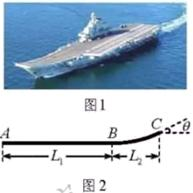
\includegraphics[width=0.3\linewidth]{picture/screenshot027}
\end{figure}


\banswer{
\begin{enumerate}
\renewcommand{\labelenumi}{\arabic{enumi}.}
% A(\Alph) a(\alph) I(\Roman) i(\roman) 1(\arabic)
%设定全局标号series=example	%引用全局变量resume=example
%[topsep=-0.3em,parsep=-0.3em,itemsep=-0.3em,partopsep=-0.3em]
%可使用leftmargin调整列表环境左边的空白长度 [leftmargin=0em]
\item
$W=7.5 \times 10^{4} \ \mathrm{J}$

\item 
$F_{\mathrm{N}}=1.1 \times 10^{3} \ \mathrm{N}$

\end{enumerate}


}





\item
\exwhere{$ 2016 $ 年上海卷}
$ 25 $.地面上物体在变力 $ F $ 作用下由静止开始竖直向上运动,力 $ F $ 随高度 $ x $ 的变化关
系如图所示,物体能上升的最大高为 $ h $,$ h<H $。当物体加速度
最大时其高度为
\tk{$ 0 $ 或 $h$},加速度的最大值为
\tk{$\frac{g h}{2 H-h}$} 
。
\begin{figure}[h!]
\centering
\includesvg[width=0.23\linewidth]{picture/svg/GZ-3-tiyou-0378}
\end{figure}





\newpage
\item
\exwhere{$ 2016 $ 年新课标 \lmd{1} 卷}
如图,一带负电荷的油滴在匀强电场中运动,其轨迹在竖直面(纸面)
内,且相对于过轨迹最低点 $ P $ 的竖直线对称。忽略空气阻力。由此可知 \xzanswer{AB} 
\begin{figure}[h!]
\centering
\includesvg[width=0.23\linewidth]{picture/svg/GZ-3-tiyou-0379}
\end{figure}




\fourchoices
{$ Q $ 点的电势比 $ P $ 点高}
{油滴在 $ Q $ 点的动能比它在 $ P $ 点的大}
{油滴在 $ Q $ 点的电势能比它在 $ P $ 点的大}
{油滴在 $ Q $ 点的加速度大小比它在 $ P $ 点的小}




\item
\exwhere{$ 2017 $ 年天津卷}
“天津之眼”是一座跨河建设、桥轮合一的摩天轮,是天津市的地标之一。摩天
轮悬挂透明座舱,乘客随座舱在竖直面内做匀速圆周运动。下列叙述正确的
是 \xzanswer{D} 
% TODO: \usepackage{graphicx} required
\begin{figure}[h!]
\centering
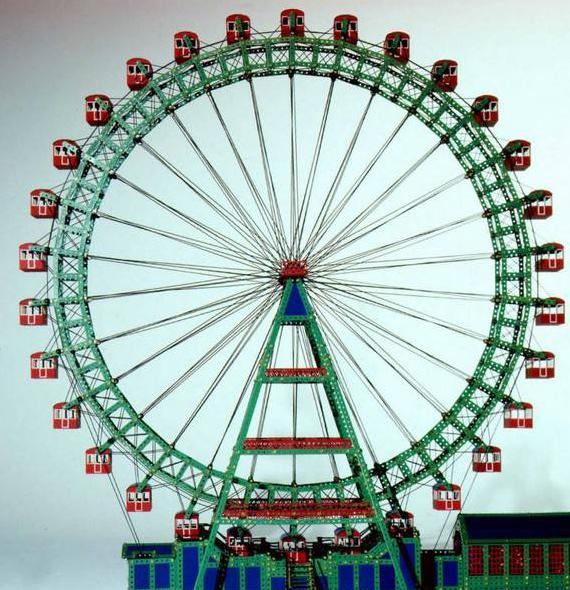
\includegraphics[width=0.2\linewidth]{picture/screenshot028}
\end{figure}

\fourchoices
{摩天轮转动过程中,乘客的机械能保持不变}
{在最高点,乘客重力大于座椅对他的支持力}
{摩天轮转动一周的过程中,乘客重力的冲量为零}
{摩天轮转动过程中,乘客重力的瞬时功率保持不变}


\newpage
\item 
\exwhere{$ 2016 $ 年天津卷}
我国将于 $ 2022 $ 年举办冬奥会,跳台滑雪是其中最具观赏性的项目之一,如图
所示。质量 $ m=60 \ kg $ 的运动员从长直助滑道 $ AB $ 的 $ A $
处由静止开始以加速度 $ a=3.6 \ m/s^{2} $ 匀加速滑下,到达
助滑道末端 $ B $ 时速度 $ v_{B} =24 \ m/s $,$ A $ 与 $ B $ 的竖直高度差
$ H=48 \ m $,为了改变运动员的运动方向,在助滑道与起
跳台之间用一段弯曲滑道衔接,其中最低点 $ C $ 处附近
是一段以 $ O $ 为圆心的圆弧。助滑道末端 $ B $ 与滑道最低
点 $ C $ 的高度差 $ h=5 \ m $,运动员在 $ B $、$ C $ 间运动时阻力做功 $ W=-1530 \ J $,取 $ g=10 \ m/s^{2} $。
\begin{enumerate}
\renewcommand{\labelenumi}{\arabic{enumi}.}
% A(\Alph) a(\alph) I(\Roman) i(\roman) 1(\arabic)
%设定全局标号series=example	%引用全局变量resume=example
%[topsep=-0.3em,parsep=-0.3em,itemsep=-0.3em,partopsep=-0.3em]
%可使用leftmargin调整列表环境左边的空白长度 [leftmargin=0em]
\item
求运动员在 $ AB $ 段下滑时受到阻力 $ F_{f} $ 的大小;
\item 
若运动员能够承受的最大压力为其所受重力的 $ 6 $ 倍,则 $ C $ 点所在圆弧的半径 $ R $ 至少应为多
大。



\end{enumerate}
\begin{figure}[h!]
\flushright
\includesvg[width=0.35\linewidth]{picture/svg/GZ-3-tiyou-0380}
\end{figure}


\banswer{
\begin{enumerate}
\renewcommand{\labelenumi}{\arabic{enumi}.}
% A(\Alph) a(\alph) I(\Roman) i(\roman) 1(\arabic)
%设定全局标号series=example	%引用全局变量resume=example
%[topsep=-0.3em,parsep=-0.3em,itemsep=-0.3em,partopsep=-0.3em]
%可使用leftmargin调整列表环境左边的空白长度 [leftmargin=0em]
\item
$ 144 \ N $

\item 
$ 12.5 \ m $



\end{enumerate}


}




\newpage
\item 
\exwhere{$ 2012 $ 年理综全国卷}
一探险队员在探险时遇到一山沟,山沟的一侧竖直,另一侧的坡面呈抛物线形状。此
队员从山沟的竖直一侧,以速度 $ v_{0} $ 沿水平方向跳向另一侧坡
面。如图所示,以沟底的 $ O $ 点为原点建立坐标系 $ Oxy $。已知,
山沟竖直一侧的高度为 $ 2 h $,坡面的抛物线方程为 $y=\frac{1}{2 h} x^{2}$,
探险队员的质量为 $ m $。人视为质点,忽略空气阻力,重力加速
度为 $ g $。
\begin{enumerate}
\renewcommand{\labelenumi}{\arabic{enumi}.}
% A(\Alph) a(\alph) I(\Roman) i(\roman) 1(\arabic)
%设定全局标号series=example	%引用全局变量resume=example
%[topsep=-0.3em,parsep=-0.3em,itemsep=-0.3em,partopsep=-0.3em]
%可使用leftmargin调整列表环境左边的空白长度 [leftmargin=0em]
\item
求此人落到坡面时的动能;

\item 
此人水平跳出的速度为多大时,他落在坡面时的动能最小?动能的最小值为多少?



\end{enumerate}
\begin{figure}[h!]
\flushright
\includesvg[width=0.38\linewidth]{picture/svg/GZ-3-tiyou-0382}
\end{figure}



\banswer{
\begin{enumerate}
\renewcommand{\labelenumi}{\arabic{enumi}.}
% A(\Alph) a(\alph) I(\Roman) i(\roman) 1(\arabic)
%设定全局标号series=example	%引用全局变量resume=example
%[topsep=-0.3em,parsep=-0.3em,itemsep=-0.3em,partopsep=-0.3em]
%可使用leftmargin调整列表环境左边的空白长度 [leftmargin=0em]
\item
$\frac{1}{2} m v^{2}=\frac{1}{2} m\left(v_{0}^{2}+\frac{4 g^{2} h^{2}}{v_{0}^{2}+g h}\right)$

\item 
$E_{k \min }=\frac{5}{2} m g h-\frac{2 m g^{2} h^{2}}{v_{0}^{2}+g h}=\frac{3}{2} m g h$


\end{enumerate}


}



\newpage
\item
\exwhere{$ 2012 $ 年理综广东卷}
图($ a $)所示的装置中,小物块 $ A $、$ B $ 质量均为 $ m $,水平面上 $ PQ $ 段长为 $ l $,与物块间的动摩擦
因数为$ \mu $,其余段光滑。初始时,挡板上的轻质弹簧处于原长;长为 $ r $ 的连杆位于图中虚线位置;$ A $
紧靠滑杆($ A $、$ B $ 间距大于 $ 2r $)
。随后,连杆以角速度$ \omega $匀速转动,带动滑杆作水平运动,滑杆的速
度$ - $时间图像如图($ b $)所示。$ A $ 在滑杆推动下运动,并在脱离滑杆后与静止的 $ B $ 发生完全非弹性
碰撞。
\begin{enumerate}
\renewcommand{\labelenumi}{\arabic{enumi}.}
% A(\Alph) a(\alph) I(\Roman) i(\roman) 1(\arabic)
%设定全局标号series=example	%引用全局变量resume=example
%[topsep=-0.3em,parsep=-0.3em,itemsep=-0.3em,partopsep=-0.3em]
%可使用leftmargin调整列表环境左边的空白长度 [leftmargin=0em]
\item
求 $ A $ 脱离滑杆时的速度 $ u_o $,及 $ A $ 与 $ B $ 碰撞过程的机械能损失$ \Delta E $。


\item 
如果 $ AB $ 不能与弹簧相碰,设 $ AB $ 从 $ P $ 点到运动停止所用的时间为 $ t_{1} $,求$ \omega $的取值范围,及 $ t_{1} $
与$ \omega $的关系式。

\item 
如果 $ AB $ 能与弹簧相碰,但不能返回道 $ P $ 点左侧,设每次压缩弹簧过程中弹簧的最大弹性势
能为 $ E_{p} $,求$ \omega $的取值范围,及 $ E_{p} $ 与$ \omega $的关系式(弹簧始终在弹性限度内)
。



\end{enumerate}
\begin{figure}[h!]
\flushright
\includesvg[width=0.75\linewidth]{picture/svg/GZ-3-tiyou-0383}
\end{figure}



\banswer{
\begin{enumerate}
\renewcommand{\labelenumi}{\arabic{enumi}.}
% A(\Alph) a(\alph) I(\Roman) i(\roman) 1(\arabic)
%设定全局标号series=example	%引用全局变量resume=example
%[topsep=-0.3em,parsep=-0.3em,itemsep=-0.3em,partopsep=-0.3em]
%可使用leftmargin调整列表环境左边的空白长度 [leftmargin=0em]
\item
$\Delta E=\frac{1}{4} m r^{2} \omega^{2}$

\item 
解得 $0<\omega \leq \frac{4 l}{r t_{1}} \quad$ 即 $0<\omega \leq \frac{2 \sqrt{2 \mu g l}}{r} \quad t_{1}=\frac{\omega r}{2 \mu g}$
\item 
$E_{p}=\frac{m\left(\omega^{2} r^{2}-8 \mu g l\right)}{4}$
\end{enumerate}


}

\newpage
\item 
\exwhere{$ 2012 $年理综山东卷}
如图所示,一工件置于水平地面上,其$ AB $段为一半径$ R=1.0 \ m $的光滑圆弧轨道,$ BC $段
为一长度$ L=0.5 \ m $的粗糙水平轨道,二者相切于$ B $点,整个轨道位于同一竖直平面内,$ P $点为圆弧轨
道上的一个确定点。一可视为质点的物块,其质量$ m=0.2 \ kg $,与$ BC $间的动摩擦因数$ \mu _{1}=0.4 $。工件质
量$ M=0.8 \ kg $,与地面间的动摩擦因数$ \mu _{2}=0.1 $。(取$ g=10 \ m/s^{2} $)
\begin{enumerate}
\renewcommand{\labelenumi}{\arabic{enumi}.}
% A(\Alph) a(\alph) I(\Roman) i(\roman) 1(\arabic)
%设定全局标号series=example	%引用全局变量resume=example
%[topsep=-0.3em,parsep=-0.3em,itemsep=-0.3em,partopsep=-0.3em]
%可使用leftmargin调整列表环境左边的空白长度 [leftmargin=0em]
\item
若工件固定,将物块由$ P $点无初速度释放,滑至$ C $点
时恰好静止,求$ P $、$ C $ 两点间的高度差$ h $。

\item 
若将一水平恒力$ F $作用于工件,使物块在$ P $点与工件
保持相对静止,一起向左做匀加速直线运动。

\begin{enumerate}
\renewcommand{\labelenumiii}{\alph{enumiii}.}
% A(\Alph) a(\alph) I(\Roman) i(\roman) 1(\arabic)
%设定全局标号series=example	%引用全局变量resume=example
%[topsep=-0.3em,parsep=-0.3em,itemsep=-0.3em,partopsep=-0.3em]
%可使用leftmargin调整列表环境左边的空白长度 [leftmargin=0em]
\item
求$ F $的大小;

\item 
当速度$ v=5 \ m/s $时,使工件立刻停止运动(即不考虑减速的时间和位移),物块飞离圆弧轨道落至
$ BC $段,求物块的落点与$ B $点间的距离。




\end{enumerate}





\end{enumerate}
\begin{figure}[h!]
\flushright
\includesvg[width=0.4\linewidth]{picture/svg/GZ-3-tiyou-0384}
\end{figure}


\banswer{
\begin{enumerate}
\renewcommand{\labelenumi}{\arabic{enumi}.}
% A(\Alph) a(\alph) I(\Roman) i(\roman) 1(\arabic)
%设定全局标号series=example	%引用全局变量resume=example
%[topsep=-0.3em,parsep=-0.3em,itemsep=-0.3em,partopsep=-0.3em]
%可使用leftmargin调整列表环境左边的空白长度 [leftmargin=0em]
\item
$h=0.2 \ \mathrm{m}$

\item 
$F=8.5 \mathrm{N}$
 \qquad $x_{2}=0.4 \mathrm{m}$

\end{enumerate}


}

\newpage
\item 
\exwhere{$ 2012 $ 年理综安徽卷}
如图所示,装置的左边是足够长的光滑水平台面,一轻质弹簧左端固定,右端连接着质量 $ M=2 \ kg $
的小物块 $ A $。装置的中间是水平传送带,
它与左右两边的台面等高,并能平滑对
接。传送带始终以 $ \mu=2 \ m/s $ 的速度逆时针转
动。装置的右边是一光滑的曲面,质量
$ m=1 \ kg $ 的小物块 $ B $ 从其上距水平台面
$ h=1.0 \ m $ 处由静止释放。已知物块 $ B $ 与传送带之间的摩擦因数$ \mu =0.2,l=1.0 \ m $。设物块 $ A $、$ B $ 间发生的
是对心弹性碰撞,第一次碰撞前物块 $ A $ 静止且处于平衡状态。取 $ g=10 \ m/s^{2} $。
\begin{enumerate}
\renewcommand{\labelenumi}{\arabic{enumi}.}
% A(\Alph) a(\alph) I(\Roman) i(\roman) 1(\arabic)
%设定全局标号series=example	%引用全局变量resume=example
%[topsep=-0.3em,parsep=-0.3em,itemsep=-0.3em,partopsep=-0.3em]
%可使用leftmargin调整列表环境左边的空白长度 [leftmargin=0em]
\item
求物块 $ B $ 与物块 $ A $ 第一次碰撞前的速度大小;
\item 
通过计算说明物块 $ B $ 与物块 $ A $ 第一次碰撞后能否运动到右边曲面上?
\item 
如果物块 $ A $、$ B $ 每次碰撞后,物块 $ A $ 再回到平衡位置时都会立即被锁定,而当他们再次碰撞
前锁定被解除,试求物块 $ B $ 第 $ n $ 次碰撞后的运动速度大小。



\end{enumerate}
\begin{figure}[h!]
\flushright
\includesvg[width=0.45\linewidth]{picture/svg/GZ-3-tiyou-0385}
\end{figure}


\banswer{
\begin{enumerate}
\renewcommand{\labelenumi}{\arabic{enumi}.}
% A(\Alph) a(\alph) I(\Roman) i(\roman) 1(\arabic)
%设定全局标号series=example	%引用全局变量resume=example
%[topsep=-0.3em,parsep=-0.3em,itemsep=-0.3em,partopsep=-0.3em]
%可使用leftmargin调整列表环境左边的空白长度 [leftmargin=0em]
\item
$ 4 \ m/s $
\item 
$x=\frac{4}{9} \mathrm{m}<1 \mathrm{m},$ 所以不能回到曲面

\item 
所以碰撞$ n $次后$ B $的速度$v_{(n+1)}$应为
$v_{n+1}=4 \cdot\left(\frac{1}{3}\right)^{n} \mathrm{m} / \mathrm{s}=\frac{4}{3^{n}} \mathrm{m} / \mathrm{s} \quad(n=0,1,2,3 \ldots \ldots)$
\end{enumerate}


}




\newpage
\item
\exwhere{$ 2012 $ 年理综四川卷}
如图所示,$ ABCD $ 为固定在竖直平面内的轨道,$ AB $ 段光滑水平,$ BC $ 段为光滑圆弧,
对应的圆心角$ \theta =37 ^{\circ} $,半径 $ r=2.5 \ m $,$ CD $ 段平直倾
斜且粗糙,各段轨道均平滑连接,倾斜轨道所在区
域有场强大小为 $ E=2 \times 10^5 \ N/C $、方向垂直于斜轨向下
的匀强电场。质量 $ m=5 \times 10^{-2} \ kg $、电荷量 $ q=+1 \times 10^{-6} \ C $
的小物体(视为质点)被弹簧枪发射后,沿水平轨
道向左滑行,在 $ C $ 点以速度 $ v_{0} =3 \ m/s $ 冲上斜轨。以
小物体通过 $ C $ 点时为计时起点,$ 0.1 \ s $ 以后,场强大小不变,方向反向。已知斜轨与小物体间的动摩
擦因数$ \mu =0.25 $。设小物体的电荷量保持不变,取 $ g=10 \ m/s^{2} $.$ \sin 37 ^{\circ} =0.6 $,$ \cos 37 ^{\circ} =0.8 $。
\begin{enumerate}
\renewcommand{\labelenumi}{\arabic{enumi}.}
% A(\Alph) a(\alph) I(\Roman) i(\roman) 1(\arabic)
%设定全局标号series=example	%引用全局变量resume=example
%[topsep=-0.3em,parsep=-0.3em,itemsep=-0.3em,partopsep=-0.3em]
%可使用leftmargin调整列表环境左边的空白长度 [leftmargin=0em]
\item
求弹簧枪对小物体所做的功;



\item 
在斜轨上小物体能到达的最高点为 $ P $,求 $ CP $ 的长度。



\end{enumerate}
\begin{figure}[h!]
\flushright
\includesvg[width=0.4\linewidth]{picture/svg/GZ-3-tiyou-0386}
\end{figure}


\banswer{
\begin{enumerate}
\renewcommand{\labelenumi}{\arabic{enumi}.}
% A(\Alph) a(\alph) I(\Roman) i(\roman) 1(\arabic)
%设定全局标号series=example	%引用全局变量resume=example
%[topsep=-0.3em,parsep=-0.3em,itemsep=-0.3em,partopsep=-0.3em]
%可使用leftmargin调整列表环境左边的空白长度 [leftmargin=0em]
\item
$W_{f}=0.475 \mathrm{J}$
\item 
$\mathrm{s}=0.57 \mathrm{m}$

\end{enumerate}


}


\newpage
\item 
\exwhere{$ 2012 $ 年物理海南卷}
如图,在竖直平面内有一固定光滑轨道,其中 $ AB $ 是长为 $ R $ 的
水平直轨道,$ BCD $ 是圆心为 $ O $、半径为 $ R $ 的
$ \frac{ 3 }{ 4 } $
圆弧轨道,两轨道相
切于 $ B $ 点。在外力作用下,一小球从 $ A $ 点由静止开始做匀加速直线
运动,到达 $ B $ 点时撤除外力。已知小球刚好能沿圆轨道经过最高点
$ C $,重力加速度大小为 $ g $。求:
\begin{enumerate}
\renewcommand{\labelenumi}{\arabic{enumi}.}
% A(\Alph) a(\alph) I(\Roman) i(\roman) 1(\arabic)
%设定全局标号series=example	%引用全局变量resume=example
%[topsep=-0.3em,parsep=-0.3em,itemsep=-0.3em,partopsep=-0.3em]
%可使用leftmargin调整列表环境左边的空白长度 [leftmargin=0em]
\item
小球从在 $ AB $ 段运动的加速度的大小;
\item 
小球从 $ D $ 点运动到 $ A $ 点所用的时间。



\end{enumerate}
\begin{figure}[h!]
\flushright
\includesvg[width=0.25\linewidth]{picture/svg/GZ-3-tiyou-0387}
\end{figure}

\banswer{
\begin{enumerate}
\renewcommand{\labelenumi}{\arabic{enumi}.}
% A(\Alph) a(\alph) I(\Roman) i(\roman) 1(\arabic)
%设定全局标号series=example	%引用全局变量resume=example
%[topsep=-0.3em,parsep=-0.3em,itemsep=-0.3em,partopsep=-0.3em]
%可使用leftmargin调整列表环境左边的空白长度 [leftmargin=0em]
\item
$a=\frac{5}{2} g$
\item 
$g t=v-v_{D}$

\end{enumerate}


}


\newpage
\item 
\exwhere{$ 2011 $ 年理综安徽卷}
如图所示,质量 $ M=2 \ kg $ 的滑块套在光滑的水平轨道上,质量 $ m=1 \ kg $ 的小球通过长
$ L=0.5 \ m $ 的轻质细杆与滑块上的光滑轴 $ O $ 连接,小球和轻杆可在竖直平面内绕 $ O $ 轴自由转动。开始
轻杆处于水平状态。现给小球一个竖直向上的初速度 $ v_{0} =4 \ m/s $,$ g $
取 $ 10 \ m/s^{2} $。
\begin{enumerate}
\renewcommand{\labelenumi}{\arabic{enumi}.}
% A(\Alph) a(\alph) I(\Roman) i(\roman) 1(\arabic)
%设定全局标号series=example	%引用全局变量resume=example
%[topsep=-0.3em,parsep=-0.3em,itemsep=-0.3em,partopsep=-0.3em]
%可使用leftmargin调整列表环境左边的空白长度 [leftmargin=0em]
\item 
若锁定滑块,试求小球通过最高点 $ P $ 时对轻杆的作用力大小和
方向。
\item 
若解除对滑块的锁定,试求小球通过最高点时的速度大小。
\item 
在满足⑵的条件下,试求小球击中滑块右侧轨道位置点与小球
起始位置点间的距离。




\end{enumerate}
\begin{figure}[h!]
\flushright
\includesvg[width=0.33\linewidth]{picture/svg/GZ-3-tiyou-0389}
\end{figure}

\banswer{
\begin{enumerate}
\renewcommand{\labelenumi}{\arabic{enumi}.}
% A(\Alph) a(\alph) I(\Roman) i(\roman) 1(\arabic)
%设定全局标号series=example	%引用全局变量resume=example
%[topsep=-0.3em,parsep=-0.3em,itemsep=-0.3em,partopsep=-0.3em]
%可使用leftmargin调整列表环境左边的空白长度 [leftmargin=0em]
\item
$F=2 \mathrm{N}$
\item 
$v_{2}=2 \mathrm{m} / \mathrm{s}$
\item 
$s_{1}=\frac{2}{3} \mathrm{m}$
\end{enumerate}


}





\newpage
\item
\exwhere{$ 2013 $ 年北京卷}
蹦床比赛分成预备运动和比赛动作两个阶段。最初,运动员静止站在蹦床上;在预备运动阶段,
他经过若干次蹦跳,逐渐增加上升高度,最终达到完成比赛动作所需的高度;此后,进入比赛动
作阶段。

把蹦床简化为一个竖直放置的轻弹簧,弹力大小 $ F=kx $ ($ x $ 为床面下沉的距离,$ k $ 为常量)
。质量
$ m=50 \ kg $ 的运动员静止站在蹦床上,床面下沉 $ x_{0}=0.10 \ m $;在预备运动中,假定运动员所做的总功 $ W $
全部用于其机械能;在比赛动作中,把该运动员视作质点,其每次离开床面做竖直上抛运动的腾
空时间均为$ \Delta t=2.0 \ s $,设运动员每次落下使床面压缩的最大深度均为 $ x_{1} $。取
重力加速度 $ g=10 \ m/s^{2} $,忽略空气阻力的影响。
\begin{enumerate}
\renewcommand{\labelenumi}{\arabic{enumi}.}
% A(\Alph) a(\alph) I(\Roman) i(\roman) 1(\arabic)
%设定全局标号series=example	%引用全局变量resume=example
%[topsep=-0.3em,parsep=-0.3em,itemsep=-0.3em,partopsep=-0.3em]
%可使用leftmargin调整列表环境左边的空白长度 [leftmargin=0em]
\item
求常量 $ k $,并在图中画出弹力 $ F $ 随 $ x $ 变化的示意图;
\item 
求在比赛动作中,运动员离开床面后上升的最大高度 $ h_m $;
\item 
借助 $ F-x $ 图像可以确定弹性做功的规律,在此基础上,求 $ x_{1} $ 和 $ W $ 的值。




\end{enumerate}
\begin{figure}[h!]
\flushright
\includesvg[width=0.25\linewidth]{picture/svg/GZ-3-tiyou-0390}
\end{figure}

\banswer{
\begin{enumerate}
\renewcommand{\labelenumi}{\arabic{enumi}.}
% A(\Alph) a(\alph) I(\Roman) i(\roman) 1(\arabic)
%设定全局标号series=example	%引用全局变量resume=example
%[topsep=-0.3em,parsep=-0.3em,itemsep=-0.3em,partopsep=-0.3em]
%可使用leftmargin调整列表环境左边的空白长度 [leftmargin=0em]
\item
 $k=5000 \mathrm{N} / \mathrm{m}$
 % \includesvg[width=0.23\linewidth]{picture/svg/GZ-3-tiyou-0391} 
\item 
 $h_{\mathrm{m}}=5 \mathrm{m}$
\item 
 $x_{1}=1.1 \mathrm{m} \quad W=2525 \mathrm{J}$



\end{enumerate}


}


\newpage
\item 
\exwhere{$ 2013 $ 年上海卷}
如图,质量为 $ M $、长为 $ L $、高为 $ h $ 的矩形滑块置于水
平地面上,滑块与地面间动摩擦因数为$ \mu $;滑块上表面光滑,其
右端放置一个质量为 $ m $ 的小球。用水平外力击打滑块左端,使
其在极短时间内获得向右的速度 $ v_{0} $,经过一段时间后小球落地。
求小球落地时距滑块左端的水平距离。
\begin{figure}[h!]
\flushright
\includesvg[width=0.28\linewidth]{picture/svg/GZ-3-tiyou-0392}
\end{figure}

\banswer{
小球脱离滑块后做自由落体运动, $t=\sqrt{\frac{2 h}{g}}$\\
滑块的运动时间 $t^{\prime}=\frac{v}{\mu g}=\frac{1}{\mu g} \sqrt{v_{0}^{2}-2 \mu\left(1+\frac{m}{M}\right) g L}$	\\
若 $t<t^{\prime}$ \quad $s=v t-\frac{1}{2} a^{\prime} t^{2}=\sqrt{\frac{2 h}{g}\left[v_{0}^{2}-2 \mu\left(1+\frac{m}{M}\right) g L\right]}-\mu h$\\
若 $t>t^{\prime}$ \quad $s^{\prime}=\frac{v_{0}^{2}}{2 \mu g}-\left(1+\frac{m}{M}\right) L$
}


\newpage
\item 
\exwhere{$ 2013 $ 年重庆卷}
在一种新的“子母球”表演中,让同一竖直线上的小球 $ A $ 和小球 $ B $,从距水平地面高度
为 $ ph $($ p > 1 $)和 $ h $ 的地方同时由静止释放,如题 $ 9 $ 图所示。球 $ A $ 的质量为 $ m $,球 $ B $ 的质量为 $ 3 \ m $。
设所有碰撞都是弹性碰撞,重力加速度大小为 $ g $,忽略球的直径、空气阻力及碰撞时间。
\begin{enumerate}
\renewcommand{\labelenumi}{\arabic{enumi}.}
% A(\Alph) a(\alph) I(\Roman) i(\roman) 1(\arabic)
%设定全局标号series=example	%引用全局变量resume=example
%[topsep=-0.3em,parsep=-0.3em,itemsep=-0.3em,partopsep=-0.3em]
%可使用leftmargin调整列表环境左边的空白长度 [leftmargin=0em]
\item
求球 $ B $ 第一次落地时球 $ A $ 的速度大小;

\item 
若球 $ B $ 在第一次上升过程中就能与球 $ A $ 相碰,求 $ p $ 的取值范围;
\item 
在⑵情形下,要使球 $ A $ 第一次碰后能到达比其释放点更高的位置,求
$ p $ 应满足的条件。



\end{enumerate}
\begin{figure}[h!]
\flushright
\includesvg[width=0.15\linewidth]{picture/svg/GZ-3-tiyou-0393}
\end{figure}

\banswer{
\begin{enumerate}
\renewcommand{\labelenumi}{\arabic{enumi}.}
% A(\Alph) a(\alph) I(\Roman) i(\roman) 1(\arabic)
%设定全局标号series=example	%引用全局变量resume=example
%[topsep=-0.3em,parsep=-0.3em,itemsep=-0.3em,partopsep=-0.3em]
%可使用leftmargin调整列表环境左边的空白长度 [leftmargin=0em]
\item
$v=\sqrt{2 g h}$
\item 
$1<p<5$
\item 
$0<p<3$
\end{enumerate}


}


\newpage
\item 
\exwhere{$ 2013 $ 年海南卷}
一质量 $ m=0.6 \ kg $ 的物体以 $ v_{0} =20 \ m/s $ 的初速度从倾角为 $ 30 ^{\circ} $ 的斜坡底端沿斜坡向上运动。当物体
向上滑到某一位置时,其动能减少了$ \Delta E_{k} =18 \ J $,机械能减少了$ \Delta E=3 \ J $,不计空气阻力,重力加速度
$ g=10 \ m/s^{2} $,求:
\begin{enumerate}
\renewcommand{\labelenumi}{\arabic{enumi}.}
% A(\Alph) a(\alph) I(\Roman) i(\roman) 1(\arabic)
%设定全局标号series=example	%引用全局变量resume=example
%[topsep=-0.3em,parsep=-0.3em,itemsep=-0.3em,partopsep=-0.3em]
%可使用leftmargin调整列表环境左边的空白长度 [leftmargin=0em]
\item
物体向上运动时加速度的大小;
\item 
物体返回斜坡底端时的动能。




\end{enumerate}

\banswer{
\begin{enumerate}
\renewcommand{\labelenumi}{\arabic{enumi}.}
% A(\Alph) a(\alph) I(\Roman) i(\roman) 1(\arabic)
%设定全局标号series=example	%引用全局变量resume=example
%[topsep=-0.3em,parsep=-0.3em,itemsep=-0.3em,partopsep=-0.3em]
%可使用leftmargin调整列表环境左边的空白长度 [leftmargin=0em]
\item
$6 m / s^{2}$
\item 
$80 \mathrm{J}$



\end{enumerate}


}


\newpage
\item 
\exwhere{$ 2013 $ 年浙江卷}
山谷中有三块石头和一根不可伸长的轻质青藤,其示意图如下。图中 $ A $、$ B $、$ C $、$ D $ 均为石头
的边缘点,$ O $ 为青藤的固定点,
$ h_{1} =1.8 \ m $,$ h_{2} =4.0 \ m $,$ x_{1} =4.8 \ m $,
$ x_{2} =8.0 \ m $。开始时,质量分别为
$ M=10 \ kg $ 和 $ m=2 \ kg $ 的大、小两只滇金丝
猴分别位于左边和中间的石头上,当大
猴发现小猴将受到伤害时,迅速从左边
石头的 $ A $ 点水平跳至中间石头,大猴抱起小猴跑到 $ C $ 点,抓住青藤下端荡到右边石头上的 $ D $ 点,
此时速度恰好为零。运动过程中猴子均看成质点,空气阻力不计,重力加速度 $ g=10 \ m/s^{2} $。求:
\begin{enumerate}
\renewcommand{\labelenumi}{\arabic{enumi}.}
% A(\Alph) a(\alph) I(\Roman) i(\roman) 1(\arabic)
%设定全局标号series=example	%引用全局变量resume=example
%[topsep=-0.3em,parsep=-0.3em,itemsep=-0.3em,partopsep=-0.3em]
%可使用leftmargin调整列表环境左边的空白长度 [leftmargin=0em]
\item
大猴从 $ A $ 点水平跳离时速度的最小值;
\item 
猴子抓住青藤荡起时的速度大小;
\item 
猴子荡起时,青藤对猴子的拉力大小。



\end{enumerate}
\begin{figure}[h!]
\flushright
\includesvg[width=0.45\linewidth]{picture/svg/GZ-3-tiyou-0395}
\end{figure}

\banswer{
\begin{enumerate}
\renewcommand{\labelenumi}{\arabic{enumi}.}
% A(\Alph) a(\alph) I(\Roman) i(\roman) 1(\arabic)
%设定全局标号series=example	%引用全局变量resume=example
%[topsep=-0.3em,parsep=-0.3em,itemsep=-0.3em,partopsep=-0.3em]
%可使用leftmargin调整列表环境左边的空白长度 [leftmargin=0em]
\item
$v_{\min }=8 \mathrm{m} / \mathrm{s}$
\item 
$v_{c}=\sqrt{2 g h_{2}}=\sqrt{80} m / s \approx 9 m / s$
\item 
$F_{T}=(M+m) g+(M+m) \frac{v_{c}^{2}}{L}=216 N$
\end{enumerate}


}


\newpage
\item 
\exwhere{$ 2013 $ 年福建卷}
如图,一不可伸长的轻绳上端悬挂于 $ O $ 点,下端系一质量 $ m=1.0 \ kg $ 的小球。现将小球
拉到 $ A $ 点(保持绳绷直)由静止释放,当它经过 $ B $ 点时绳恰好被
拉断,小球平抛后落在水平地面上的 $ C $ 点。地面上的 $ D $ 点与 $ OB $
在同一竖直线上,已知绳长 $ L=1.0 \ m $,$ B $ 点离地高度 $ H=1.0 \ m $,
$ A $、$ B $ 两点的高度差 $ h=0.5 \ m $,重力加速度 $ g $ 取 $ 10 \ m/s^{2} $,不计空气
影响,求:
\begin{enumerate}
\renewcommand{\labelenumi}{\arabic{enumi}.}
% A(\Alph) a(\alph) I(\Roman) i(\roman) 1(\arabic)
%设定全局标号series=example	%引用全局变量resume=example
%[topsep=-0.3em,parsep=-0.3em,itemsep=-0.3em,partopsep=-0.3em]
%可使用leftmargin调整列表环境左边的空白长度 [leftmargin=0em]
\item
地面上 $ DC $ 两点间的距离 $ s $;

\item 
轻绳所受的最大拉力大小。



\end{enumerate}
\begin{figure}[h!]
\flushright
\includesvg[width=0.25\linewidth]{picture/svg/GZ-3-tiyou-0396}
\end{figure}


\banswer{
\begin{enumerate}
\renewcommand{\labelenumi}{\arabic{enumi}.}
% A(\Alph) a(\alph) I(\Roman) i(\roman) 1(\arabic)
%设定全局标号series=example	%引用全局变量resume=example
%[topsep=-0.3em,parsep=-0.3em,itemsep=-0.3em,partopsep=-0.3em]
%可使用leftmargin调整列表环境左边的空白长度 [leftmargin=0em]
\item
$ s=1.41 \mathrm{m}$
\item 
$F=20 \mathrm{N}$



\end{enumerate}


}


\newpage
\item 
\exwhere{$ 2011 $ 年理综广东卷}
如图所示,以 $ A $、$ B $ 和 $ C $、$ D $ 为端点的两半圆形光滑轨道固定于竖直平面内,一滑板
静止在光滑水平地面上,左端紧靠 $ B $ 点,上表面所在平面与两半圆分别相切于 $ B $、$ C $。一物块被轻
放在水平匀速运动的传送带上 $ E $ 点,运动到 $ A $ 时刚好与传送带速度相同,然后经 $ A $ 沿半圆轨道滑
下,再经 $ B $ 滑上滑板。滑板运动到 $ C $ 时被牢固粘连。物块可视为质点,质量为 $ m $,滑板质量
$ M=2 \ m $,两半圆半径均为 $ R $,板长 $ l=6.5R $,板右端到 $ C $ 的距离 $ L $ 在 $ R < L < 5R $ 范围内取值。$ E $ 距 $ A $
为 $ s=5R $。物块与传送带、物块与滑板间的动摩擦因素均为$ \mu =0.5 $,重力加速度取 $ g $。
\begin{enumerate}
\renewcommand{\labelenumi}{\arabic{enumi}.}
% A(\Alph) a(\alph) I(\Roman) i(\roman) 1(\arabic)
%设定全局标号series=example	%引用全局变量resume=example
%[topsep=-0.3em,parsep=-0.3em,itemsep=-0.3em,partopsep=-0.3em]
%可使用leftmargin调整列表环境左边的空白长度 [leftmargin=0em]
\item
求物块滑到 $ B $ 点的速度大小;
\item 
试讨论物块从滑上滑板到离开滑板右端的过程中,克服摩擦力做的功 $ Wf $ 与 $ L $ 的关系,并判断
物块能否滑到 $ CD $ 轨道的中点。



\end{enumerate}
\begin{figure}[h!]
\flushright
\includesvg[width=0.65\linewidth]{picture/svg/GZ-3-tiyou-0397}
\end{figure}


\banswer{
\begin{enumerate}
\renewcommand{\labelenumi}{\arabic{enumi}.}
% A(\Alph) a(\alph) I(\Roman) i(\roman) 1(\arabic)
%设定全局标号series=example	%引用全局变量resume=example
%[topsep=-0.3em,parsep=-0.3em,itemsep=-0.3em,partopsep=-0.3em]
%可使用leftmargin调整列表环境左边的空白长度 [leftmargin=0em]
\item
$v_{B}=3 \sqrt{g R}$

\item 
滑块不可能滑到CD轨道的中点。
\end{enumerate}


}


\newpage
\item 
\exwhere{$ 2011 $ 年理综福建卷}
如图为某种鱼饵自动投放器中的投饵管装置示意图,其下半
部 $ AB $ 是一长为 $ 2R $ 的竖直细管,上半部 $ BC $ 是半径为 $ R $ 的四分之一圆弧
弯管,管口沿水平方向,$ AB $ 管内有一原长为 $ R $、下端固定的轻质弹簧。
投饵时,每次总将弹簧长度压缩到 $ 0.5R $ 后锁定,在弹簧上端放置一粒鱼
饵,解除锁定,弹簧可将鱼饵弹射出去。设质量为 $ m $ 的鱼饵到达管口 $ C $
时,对管壁的作用力恰好为零。不计鱼饵在运动过程中的机械能损失,且
锁定和解除锁定时,均不改变弹簧的弹性势能。已知重力加速度为 $ g $。
求:
\begin{enumerate}
\renewcommand{\labelenumi}{\arabic{enumi}.}
% A(\Alph) a(\alph) I(\Roman) i(\roman) 1(\arabic)
%设定全局标号series=example	%引用全局变量resume=example
%[topsep=-0.3em,parsep=-0.3em,itemsep=-0.3em,partopsep=-0.3em]
%可使用leftmargin调整列表环境左边的空白长度 [leftmargin=0em]
\item
质量为 $ m $ 的鱼饵到达管口 $ C $ 时的速度大小 $ v_{1} $;
\item 
弹簧压缩到 $ 0.5R $ 时的弹性势能 $ E_{p} $;
\item 
已知地面与水面相距 $ 1.5R $,若使该投饵管绕 $ AB $ 管的中轴线 $ OO ^{\prime} $在 $ 90 \degree $角的范围内来回缓慢转
动,每次弹射时只放置一粒鱼饵,鱼饵的质量在 $ \frac{ 2 }{ 3 } \ m $ 到 $ m $ 之间变化,且均能落到水面。持续投放
足够长时间后,鱼饵能够落到水面的最大面积 $ S $ 是多少?




\end{enumerate}
\begin{figure}[h!]
\flushright
\includesvg[width=0.25\linewidth]{picture/svg/GZ-3-tiyou-0398}
\end{figure}


\banswer{
\begin{enumerate}
\renewcommand{\labelenumi}{\arabic{enumi}.}
% A(\Alph) a(\alph) I(\Roman) i(\roman) 1(\arabic)
%设定全局标号series=example	%引用全局变量resume=example
%[topsep=-0.3em,parsep=-0.3em,itemsep=-0.3em,partopsep=-0.3em]
%可使用leftmargin调整列表环境左边的空白长度 [leftmargin=0em]
\item
 $\sqrt{g R}$
\item 
$3 m g R$
\item 
$\frac{33}{4} \pi R^{3}$



\end{enumerate}


}


\newpage
\item 
\exwhere{$ 2011 $ 年理综全国卷}
装甲车和战舰 采用多层钢板比采用同样质量的单层钢板更能抵御穿甲弹的射击。通过
对一下简化模型的计算可以粗略说明其原因。质量为 $ 2 \ m $、厚度为 $ 2d $
的钢板静止在水平光滑桌面上。质量为 $ m $ 的子弹以某一速度垂直射
向该钢板,刚好能将钢板射穿。现把钢板分成厚度均为 $ d $、质量均为
$ m $ 的相同两块,间隔一段距离水平放置,如图所示。若子弹以相同的
速度垂直射向第一块钢板,穿出后再射向第二块钢板,求子弹射入第二块钢板的深度。设子弹在
钢板中受到的阻力为恒力,且两块钢板不会发生碰撞。不计重力影响。
\begin{figure}[h!]
\flushright
\includesvg[width=0.35\linewidth]{picture/svg/GZ-3-tiyou-0399}
\end{figure}

\banswer{
$x=\frac{1}{2}\left(1+\frac{\sqrt{3}}{2}\right) d$
}




\end{enumerate}

